\section{Agent Architectures and Planning}

\begin{frame}{}
    \LARGE Agentic Models: \textbf{Architectures and Planning}

    \vspace{1em}
    \normalsize ReAct gave us the loop. What did the next three years add to it, and what did they remove?
\end{frame}

\begin{frame}{Two Axes Beyond ReAct}
    \centering
    \begin{adjustbox}{max width=\linewidth}\begin{tikzpicture}[font=\footnotesize,
        cell/.style={draw, rounded corners=2pt, minimum width=2.75cm, minimum height=0.85cm, align=center},
        ax/.style={-{Stealth}, thick, gray}]
        \draw[ax] (-0.3,-0.2) -- (12.4,-0.2);
        \draw[ax] (-0.3,-0.2) -- (-0.3,3.5);
        \node[gray, anchor=west] at (8.6,-0.5) {\textbf{Axis 1: control flow}};
        \node[gray, rotate=90, anchor=west] at (-0.6,0.2) {\textbf{Axis 2: action interface}};
        \node[cell, fill=gray!12] (a) at (1.4,0.5) {\textbf{Interleaved}\\ReAct};
        \node[cell, fill=KAUSTcyan!15] (b) at (4.5,0.5) {\textbf{Plan first}\\ReWOO, Plan-and-Solve};
        \node[cell, fill=KAUSTcyan!15] (c) at (7.6,0.5) {\textbf{Plan as a DAG}\\LLMCompiler};
        \node[cell, fill=KAUSTcyan!15] (d) at (10.7,0.5) {\textbf{Search}\\LATS};
        \node[cell, fill=darkorange!18] (e) at (1.4,1.8) {\textbf{Code actions}\\CodeAct};
        \node[cell, fill=darkorange!18] (f) at (1.4,3.0) {\textbf{LM-tailored commands}\\SWE-agent};
        \draw[-{Stealth}, thick] (a) -- (b);
        \draw[-{Stealth}, thick] (b) -- (c);
        \draw[-{Stealth}, thick] (c) -- (d);
        \draw[-{Stealth}, thick] (a) -- (e);
        \draw[-{Stealth}, thick] (e) -- (f);
        \node[align=left, text width=7.4cm, anchor=west] at (4.1,2.4) {\textbf{Reading the map.} Axis 1 changes \emph{when} the model thinks and acts. Axis 2 changes \emph{what an action is}.\\[0.4em] Production systems mostly moved \alert{up} axis 2 and kept a simple loop on axis 1.};
    \end{tikzpicture}\end{adjustbox}
    \vspace{0.3em}
    \begin{itemize}\itemsep0.3em
        \item JSON tool calls sit at the origin: one call, one observation, repeat.
        \item This section walks axis 1 first, then axis 2, then asks where planning went.
    \end{itemize}
    \src{Synthesis of Xu et al., \href{https://arxiv.org/abs/2305.18323}{arXiv:2305.18323}. Kim et al., \href{https://arxiv.org/abs/2312.04511}{arXiv:2312.04511}. Zhou et al., \href{https://arxiv.org/abs/2310.04406}{arXiv:2310.04406}. Wang et al., \href{https://arxiv.org/abs/2402.01030}{arXiv:2402.01030}. Yang et al., \href{https://arxiv.org/abs/2405.15793}{arXiv:2405.15793}.}
\end{frame}

\begin{frame}{Plan First: ReWOO and LLMCompiler}
    \centering
    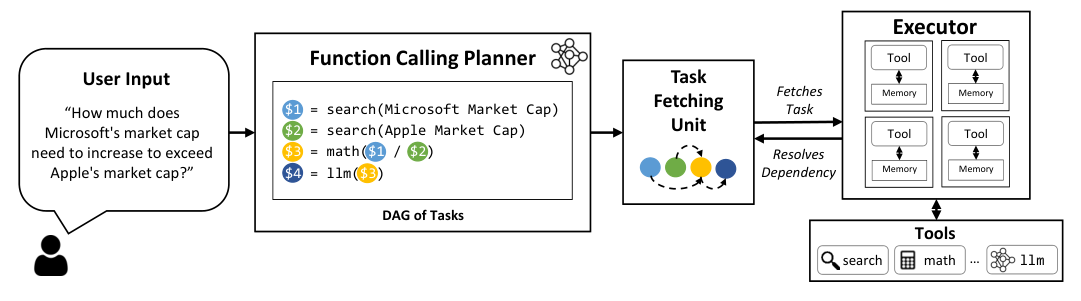
\includegraphics[width=0.92\linewidth,height=0.3\textheight,keepaspectratio]{images/agentic-models-memory/llmcompiler_fig2_overview.png}
    \begin{itemize}\itemsep0.3em
        \item \textbf{ReWOO.} ReAct re-sends its history at every tool call. Plan once instead, with placeholders for evidence. HotpotQA: \textbf{1,986 tokens} against 9,795, at similar accuracy.
        \item \textbf{LLMCompiler} (above). The plan is a DAG, executed in parallel: up to 3.7$\times$ faster and 6.7$\times$ cheaper than ReAct.
    \end{itemize}
    \caveat{\textbf{Historical numbers.} gpt-3.5-era results on short QA. Prompt caching has since weakened the token argument.}
    \src{Xu et al., ``ReWOO: Decoupling Reasoning from Observations,'' \href{https://arxiv.org/abs/2305.18323}{arXiv:2305.18323}, Table 2. Figure: Kim et al., ``An LLM Compiler for Parallel Function Calling,'' \href{https://arxiv.org/abs/2312.04511}{arXiv:2312.04511}, Figure 2.}
\end{frame}

\begin{frame}{Search Is Expensive, and Self-Checking Is Not Enough}
    \begin{columns}[T,onlytextwidth]
        \column{0.53\textwidth}
        \begin{itemize}\itemsep0.4em
            \item \textbf{LATS} runs tree search over trajectories. It needs an environment that can be \alert{reverted}:
            \[
                \mathrm{UCT}(s)=V(s)+w\sqrt{\tfrac{\ln N(p)}{N(s)}}
            \]
            \item \textbf{Can LLMs plan?} On PlanBench, o1 is a large step up but far from saturating it.
            \item \textbf{LLM-Modulo:} let the LLM \emph{generate} candidates, and let external, sound verifiers \emph{test} them.
        \end{itemize}
        \column{0.44\textwidth}
        \centering
        \small
        \begin{adjustbox}{max width=\linewidth}\begin{tabular}{lcc}
            \toprule
            \textbf{HumanEval, GPT-4} & \textbf{Acc.} & \textbf{Cost} \\
            \midrule
            \rowcolor{KAUSTcyan!12} Simple ``warming'' baseline & 93.2\% & \$2.45 \\
            Reflexion & 87.8\% & \$3.90 \\
            LATS & 88.0\% & \alert{\$134.50} \\
            \bottomrule
        \end{tabular}\end{adjustbox}

        \vspace{0.8em}
        \begin{adjustbox}{max width=\linewidth}\begin{tikzpicture}[font=\scriptsize, >=Stealth,
            b/.style={draw, rounded corners=2pt, minimum width=2.2cm, minimum height=0.6cm, align=center}]
            \node[b, fill=KAUSTcyan!20] (g) at (0,0) {LLM generates};
            \node[b, fill=darkorange!20] (v) at (3.4,0) {Verifier tests};
            \draw[->, thick] (g.north east) to[bend left=25] node[above] {candidate plan} (v.north west);
            \draw[->, thick] (v.south west) to[bend left=25] node[below] {critique} (g.south east);
        \end{tikzpicture}\end{adjustbox}
    \end{columns}
    \vspace{0.2em}
    \takeaway{In production the verifier is a \textbf{test suite, a linter or a screenshot}, not the model's own opinion. Day 2 covered search and reflection in depth.}
    \src{Zhou et al., ``Language Agent Tree Search,'' \href{https://arxiv.org/abs/2310.04406}{arXiv:2310.04406}. Kapoor et al., ``AI Agents That Matter,'' \href{https://arxiv.org/abs/2407.01502}{arXiv:2407.01502}. Valmeekam et al., \href{https://arxiv.org/abs/2409.13373}{arXiv:2409.13373}. Kambhampati et al., \href{https://arxiv.org/abs/2402.01817}{arXiv:2402.01817}.}
\end{frame}

\begin{frame}{Axis 2: Code as the Action Space}
    \centering
    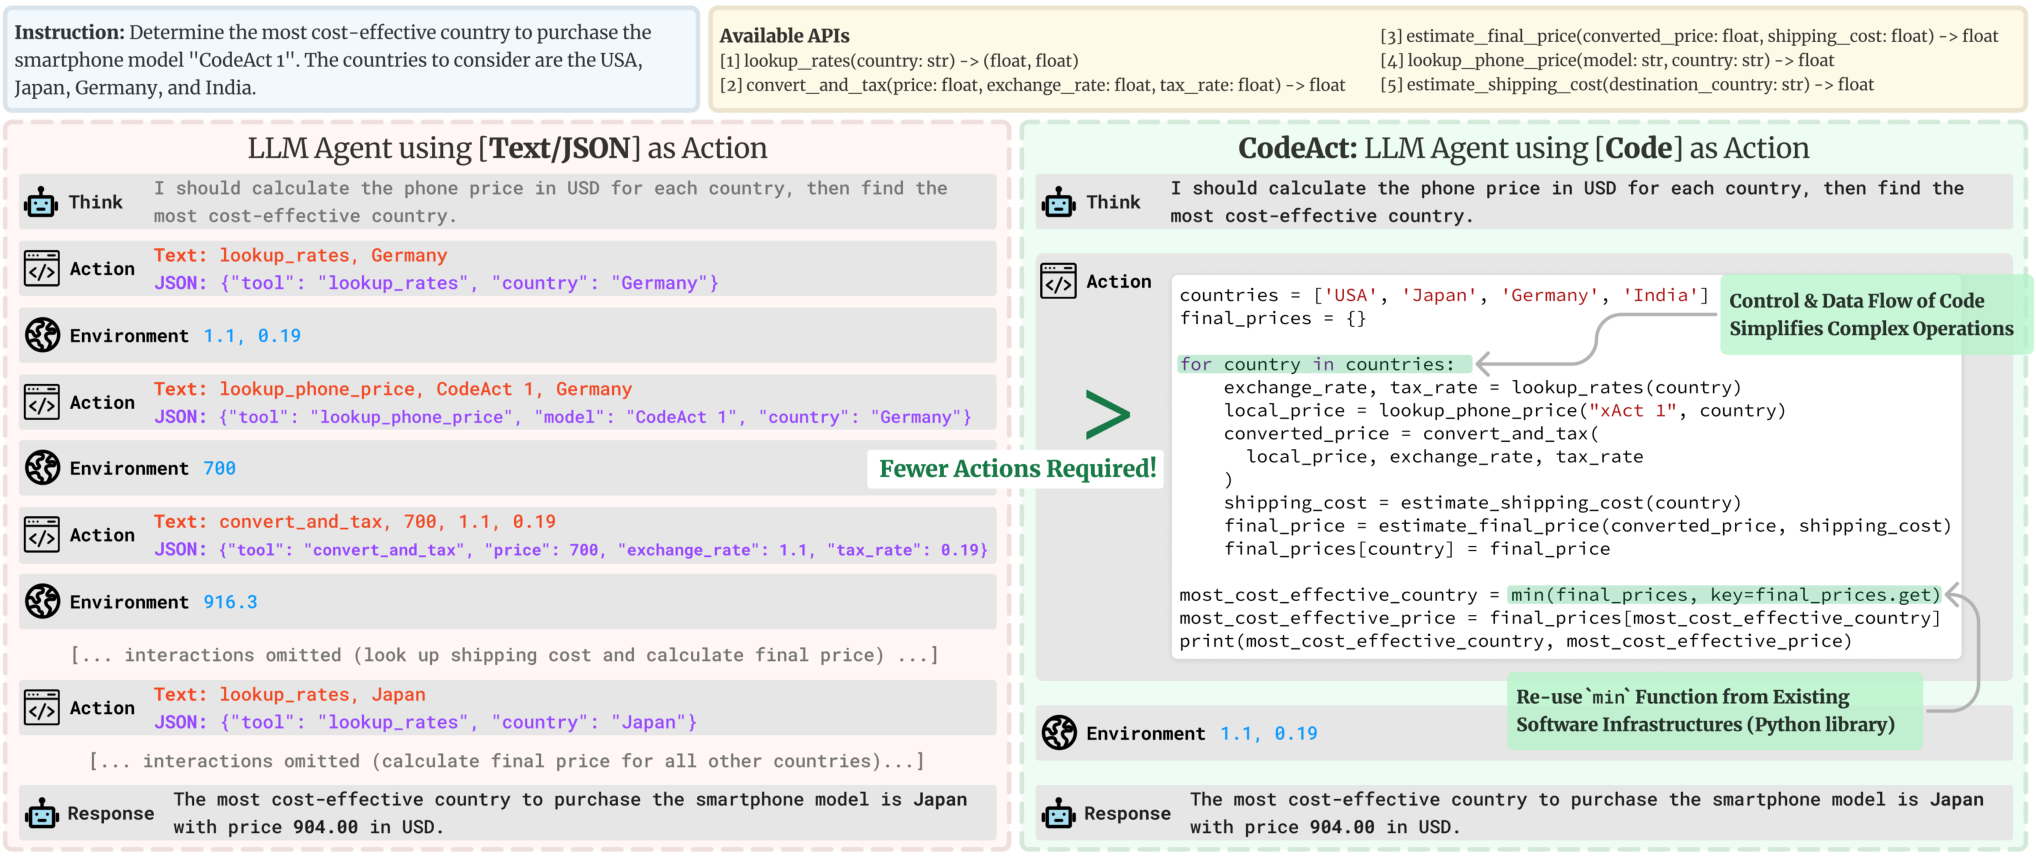
\includegraphics[width=0.9\linewidth,height=0.4\textheight,keepaspectratio]{images/agentic-models-memory/codeact_fig1_code_vs_json.png}
    \begin{itemize}\itemsep0.3em
        \item \textbf{Why.} One JSON call does one thing. A code action has loops, variables and existing libraries.
        \item \textbf{Result} (M3ToolEval, 82 multi-tool tasks): \textbf{74.4\%} success for code, against 52.4\% for JSON and 53.7\% for text, in 5.5 turns instead of 7.6.
        \item \textbf{Afterlife.} OpenHands ships a CodeAct agent. Presenting MCP servers as code APIs cut one Anthropic example from 150,000 to 2,000 tokens.
    \end{itemize}
    \src{Wang et al., ``Executable Code Actions Elicit Better LLM Agents,'' \href{https://arxiv.org/abs/2402.01030}{arXiv:2402.01030}, Figure 1. Wang et al., ``OpenHands,'' \href{https://arxiv.org/abs/2407.16741}{arXiv:2407.16741}. Anthropic, ``Code execution with MCP'' (Nov 2025).}
\end{frame}

\begin{frame}{Axis 2: The Agent-Computer Interface}
    \begin{columns}[T,onlytextwidth]
        \column{0.57\textwidth}
        \begin{itemize}\itemsep0.5em
            \item \textbf{Thesis.} An LM agent is a new kind of end user. It needs its own interface, as humans need an IDE.
            \item \textbf{SWE-agent's design rules:}
            \begin{itemize}\itemsep0.2em
                \item simple, compact actions
                \item informative but concise feedback
                \item \textbf{guardrails}: a linter rejects broken edits
            \end{itemize}
            \item A windowed file viewer and a capped search (at most 50 results) keep context small.
            \item Anthropic reports the same lesson: they spent more time on the tools than on the prompt.
        \end{itemize}
        \column{0.4\textwidth}
        \centering
        \small
        \begin{adjustbox}{max width=\linewidth}\begin{tabular}{lc}
            \toprule
            \textbf{Variant} & \textbf{SWE-bench Lite} \\
            \midrule
            \rowcolor{KAUSTcyan!12} Full interface & 18.0\% \\
            No linting & 15.0\% \\
            30-line window & 14.3\% \\
            Full-file window & 12.7\% \\
            Iterative search & 12.0\% \\
            No edit command & 10.3\% \\
            \bottomrule
        \end{tabular}\end{adjustbox}

        \vspace{0.5em}
        {\footnotesize Same model, GPT-4 Turbo. Only the interface changes.}
    \end{columns}
    \vspace{0.3em}
    \caveat{The absolute scores are from 2024. Open models now report 73 to 80\% on SWE-bench Verified. The ablation is what lasts.}
    \src{Yang et al., ``SWE-agent: Agent-Computer Interfaces Enable Automated Software Engineering,'' \href{https://arxiv.org/abs/2405.15793}{arXiv:2405.15793}, Table 3. Anthropic, ``Building Effective Agents'' (Dec 2024).}
\end{frame}

\begin{frame}{Planning Moves Into the Model}
    \begin{center}
    \small
    \renewcommand{\arraystretch}{1.2}
    \begin{adjustbox}{max width=\linewidth}\begin{tabular}{>{\raggedright\arraybackslash}p{2.6cm}>{\raggedright\arraybackslash}p{4.4cm}>{\raggedright\arraybackslash}p{6.1cm}}
        \toprule
        \textbf{Provider} & \textbf{Reasoning state} & \textbf{What the client must do} \\
        \midrule
        Anthropic & thinking blocks between tool calls & keep the blocks in the turn \\
        OpenAI Responses & reasoning items & pass them back around function calls: about +3\% on SWE-bench \\
        Google Gemini & encrypted thought signatures & echo them back unchanged \\
        Open models & \texttt{<think>} content & keep it in history. Removing it hurts (MiniMax-M2) \\
        \bottomrule
    \end{tabular}\end{adjustbox}
    \end{center}
    \begin{itemize}\itemsep0.3em
        \item The model now plans and replans \emph{in its thinking, between tool calls}. Kimi K2 Thinking stays coherent over \textbf{200 to 300} consecutive calls.
    \end{itemize}
    \takeaway{Planning-first became a trained behaviour. The price is an API contract: \textbf{preserve the reasoning state}.}
    \src{Anthropic, extended thinking docs. OpenAI, Responses API cookbook, ``Reasoning items.'' Google, Gemini thinking docs. MiniMax-M2 and Kimi K2 Thinking model cards.}
\end{frame}

\begin{frame}{From Prompt Engineering to Context Engineering}
    \begin{columns}[T,onlytextwidth]
        \column{0.62\textwidth}
        \begin{itemize}\itemsep0.45em
            \item \textbf{Context rot.} Recall degrades as context grows. Treat context as a finite \emph{attention budget}.
            \item \textbf{Four techniques:} compaction, structured notes, sub-agents that return 1 to 2 thousand token summaries, and just-in-time retrieval.
            \item \textbf{Across many windows.} An \emph{initializer} agent writes a progress file and a list of 200+ features marked pass or fail. A \emph{coding} agent then advances one feature per session.
        \end{itemize}
        \column{0.35\textwidth}
        \centering
        \begin{adjustbox}{max width=\linewidth}\begin{tikzpicture}[font=\footnotesize, >=Stealth,
            b/.style={draw, rounded corners=2pt, minimum width=2.5cm, minimum height=0.65cm, align=center}]
            \node[b, fill=KAUSTcyan!20] (g) at (0,3.0) {Gather context};
            \node[b, fill=darkorange!20] (a) at (0,1.8) {Take action};
            \node[b, fill=gray!15] (v) at (0,0.6) {Verify work};
            \draw[->, thick] (g) -- (a);
            \draw[->, thick] (a) -- (v);
            \draw[->, thick] (v.east) to[bend right=60] (g.east);
            \node[gray, font=\scriptsize] at (0,-0.1) {the Claude Agent SDK loop};
        \end{tikzpicture}\end{adjustbox}
    \end{columns}
    \vspace{0.4em}
    \takeaway{The guidance shifted from \emph{``which loop pattern?''} (2024) to \emph{``how do we manage state across many context windows?''} (late 2025).}
    \src{Anthropic: Rajasekaran et al., ``Effective context engineering for AI agents'' (Sep 2025). Young, ``Effective harnesses for long-running agents'' (Nov 2025). Shihipar, ``Building agents with the Claude Agent SDK'' (Sep 2025).}
\end{frame}

\begin{frame}{Agentic Foundation Models: The Open-Lab Recipe}
    \centering
    \begin{adjustbox}{max width=\linewidth}\begin{tikzpicture}[font=\footnotesize, >=Stealth,
        b/.style={draw, rounded corners=2pt, minimum width=3.05cm, minimum height=1.25cm, align=center, text width=2.85cm}]
        \node[b, fill=gray!12] (a) at (0,0) {\textbf{1. Synthesise}\\tools and environments};
        \node[b, fill=KAUSTcyan!18] (b) at (3.6,0) {\textbf{2. Generate}\\trajectories with simulated users and tools};
        \node[b, fill=KAUSTcyan!18] (c) at (7.2,0) {\textbf{3. Filter}\\with rubrics or an LLM judge};
        \node[b, fill=darkorange!20] (d) at (10.8,0) {\textbf{4. Reinforce}\\outcome rewards in sandboxes};
        \draw[->, thick] (a) -- (b);
        \draw[->, thick] (b) -- (c);
        \draw[->, thick] (c) -- (d);
    \end{tikzpicture}\end{adjustbox}
    \vspace{0.5em}
    \begin{itemize}\itemsep0.4em
        \item \textbf{Kimi K2.} 3,000+ real MCP tools plus 20,000+ synthetic ones, an LLM user, a \emph{stateful} tool simulator, and real sandboxes for code.
        \item \textbf{GLM-4.5.} Outcome rewards, with a format penalty that \alert{ends the trace} when a tool call fails.
        \item \textbf{DeepSeek-V3.2.} 1,800+ environments and 85,000 prompts. \textbf{Qwen3-Coder.} 20,000 parallel environments.
    \end{itemize}
    \vspace{0.2em}
    \takeaway{Day 3 covered the RL algorithms. What is new here is the \textbf{scale of environments and verifiers}.}
    \src{Recipe is a synthesis of: Kimi Team, \href{https://arxiv.org/abs/2507.20534}{arXiv:2507.20534}. GLM-4.5 Team, \href{https://arxiv.org/abs/2508.06471}{arXiv:2508.06471}. DeepSeek-AI, \href{https://arxiv.org/abs/2512.02556}{arXiv:2512.02556}. Qwen, ``Qwen3-Coder'' blog (Jul 2025).}
\end{frame}

\begin{frame}{Trained for Agency: What the Reports Show}
    \begin{columns}[T,onlytextwidth]
        \column{0.5\textwidth}
        \centering
        \begin{adjustbox}{max width=\linewidth}\begin{tikzpicture}
            \begin{axis}[
                ybar, bar width=10pt, width=7.2cm, height=5.2cm,
                ymin=30, ymax=90, ylabel={SWE-bench Verified (\%)},
                symbolic x coords={SWE-RL,DeepSWE,Kimi K2,DS-V3.2,GLM-5,M2.5},
                xtick=data, x tick label style={font=\scriptsize, rotate=30, anchor=east},
                y label style={font=\scriptsize}, y tick label style={font=\scriptsize},
                nodes near coords, nodes near coords style={font=\tiny},
                axis lines*=left, ymajorgrids, grid style={gray!20}]
                \addplot[fill=KAUSTcyan!55, draw=KAUSTcyan!70!black] coordinates {(SWE-RL,41.0) (DeepSWE,42.2) (Kimi K2,65.8) (DS-V3.2,73.1) (GLM-5,77.8) (M2.5,80.2)};
            \end{axis}
        \end{tikzpicture}\end{adjustbox}

        {\scriptsize Open models, February 2025 to early 2026.}
        \column{0.48\textwidth}
        \begin{itemize}\itemsep0.5em
            \item \textbf{Open models} roughly doubled their score in a year.
            \item \textbf{Closed labs} disclose less. Deep research was trained with RL on browsing tasks. Operator used SFT for perception, then RL.
            \item \textbf{One disclosed reward.} codex-1 often claimed success on impossible tasks. Penalising results inconsistent with its actions raised honest ``could not complete'' reports from \textbf{0.15 to 0.85}.
        \end{itemize}
    \end{columns}
    \vspace{0.3em}
    \caveat{The scaffolds differ across these reports, so this is \textbf{not} one controlled curve. Scores now also include ``context management'' in the harness.}
    \src{Wei et al., \href{https://arxiv.org/abs/2502.18449}{arXiv:2502.18449}. Together AI, DeepSWE blog. Kimi Team, \href{https://arxiv.org/abs/2507.20534}{arXiv:2507.20534}. DeepSeek-AI, \href{https://arxiv.org/abs/2512.02556}{arXiv:2512.02556}. GLM-5 and MiniMax-M2.5 model cards. OpenAI system cards: deep research, Operator, codex-1.}
\end{frame}

\begin{frame}{Does the Scaffold Still Matter?}
    \begin{center}
    \small
    \renewcommand{\arraystretch}{1.2}
    \begin{adjustbox}{max width=\linewidth}\begin{tabular}{>{\raggedright\arraybackslash}p{3.4cm}>{\raggedright\arraybackslash}p{6.0cm}>{\raggedright\arraybackslash}p{3.6cm}}
        \toprule
        \textbf{Evidence} & \textbf{Finding} & \textbf{Reading} \\
        \midrule
        METR tasks (Feb 2026) & Opus 4.5 in Claude Code beats a plain ReAct scaffold in only 50.7\% of bootstrap samples & scaffold barely matters \\
        Terminal-Bench 2.0 & Gemini 2.5 Pro: 32.6\% on Terminus 2, 15.7\% on OpenHands & scaffold changes score by \alert{2.1$\times$} \\
        Terminal-Bench 2.0 & GPT-5.3-Codex: 64.7 on Terminus 2, 77.3 on the Codex harness & vendors tune to their own models \\
        \bottomrule
    \end{tabular}\end{adjustbox}
    \end{center}
    \begin{itemize}\itemsep0.4em
        \item The Terminal-Bench authors still conclude that \emph{``model selection is usually more important than agent scaffold.''}
        \item Yu Su: \emph{``stronger LLMs may require less scaffolding (i.e., more `reactive')''}.
    \end{itemize}
    \src{METR, ``Measuring time horizon using Claude Code and Codex'' (Feb 2026). Merrill et al., ``Terminal-Bench,'' \href{https://arxiv.org/abs/2601.11868}{arXiv:2601.11868}, Table 2. Google DeepMind, Gemini 3.1 Pro Model Evaluation (Feb 2026). Su, Berkeley CS294 (Feb 2025).}
\end{frame}

\begin{frame}{Architectures: What to Remember}
    \begin{itemize}\itemsep0.6em
        \item Plan-first scaffolds and tree search are the \textbf{2023 answers}. They cut tokens or raised accuracy, at a cost that simple baselines often beat.
        \item What lasted is the \textbf{action interface}: code actions and interfaces designed for the model.
        \item Planning moved \textbf{into the model} as interleaved thinking. The client must now carry reasoning state across tool calls.
        \item Frontier agency is \textbf{trained}: synthetic tools, simulated users, judged trajectories and RL in sandboxes.
        \item The harness is part of the system, and part of the score.
    \end{itemize}
    \vspace{0.4em}
    \takeaway{\textbf{Next.} Every one of these agents acts through tools. How does a model learn to call them, and how do we know it calls them correctly?}
\end{frame}
